% docs/Latex/Task026_027_Summary.tex -- review summary of the two most recent trials (TASK-026, TASK-027).
% Every number is quoted from:
%   docs/experiments/2026-10-19_phase1_g12_tuning/{README,PHASE1_RESULTS_REPORT}.md   (TASK-20261019-026)
%   docs/experiments/2026-10-22_sample_efficiency/{README,RESULTS}.md                  (TASK-20261022-027)
%   docs/core/STATE.yaml                                                              (both task entries)
% Differences of means in the figures are arithmetic on those tables and are marked as such in the captions.
% appendix_screens.tex / appendix_perseed.tex are generated mechanically from RESULTS.md (no retyping).
\documentclass[10pt,a4paper]{article}
\usepackage[margin=2cm]{geometry}
\usepackage{booktabs,array,xcolor,amsmath,parskip,longtable,caption}
\usepackage[colorlinks=true,linkcolor=blue!50!black,urlcolor=blue!50!black]{hyperref}
\usepackage{float}
\usepackage{url}
\usepackage{tikz}
\usetikzlibrary{arrows.meta,positioning,shapes.geometric,fit,calc}
\usepackage{pgfplots}
\pgfplotsset{compat=1.16}
\captionsetup{font=small,labelfont=bf,skip=4pt}
\setlength{\tabcolsep}{4pt}
\renewcommand{\arraystretch}{1.12}
\newcommand{\p}[1]{\texttt{\small #1}}

% Okabe--Ito colour-blind-safe palette
\definecolor{cClean}{HTML}{0072B2}   % P5-clean, EP-A
\definecolor{cCont}{HTML}{D55E00}    % P5-contested
\definecolor{cDiag}{HTML}{7F7F7F}    % diagnostic, not a gate
\definecolor{cGood}{HTML}{009E73}
\definecolor{cWarn}{HTML}{E69F00}
\definecolor{cBad}{HTML}{CC3311}
\definecolor{cLine}{HTML}{222222}

\title{Summary of the Two Most Recent Trials\\[2pt]
\large TASK-026 (tuning and data-scaling diagnostic) and TASK-027 (sample-efficiency ideas)\\
Aim: gate G1.2 of Phase~1 on Craftax-Classic}
\author{Branch \p{claude/t026-sample-efficiency}; trials of 2026-10-19 and 2026-10-22}
\date{Prepared 2026-10-23 for review}

\begin{document}
\maketitle

% -------------------------------------------------------------------------------------------------
\section*{How to read this document}
\noindent\fbox{\parbox{\dimexpr\linewidth-2\fboxsep-2\fboxrule}{\small
Thank you for taking the time to review these results. The document is organised around figures; each caption states what to look at.
\textbf{Colour code used throughout:}
{\color{cClean}\rule{1.2ex}{1.2ex}}~P5-clean arm (counts as EP-A evidence),
{\color{cCont}\rule{1.2ex}{1.2ex}}~P5-contested arm (reward coefficient changed; \emph{cannot} count toward any gate),
{\color{cDiag}\rule{1.2ex}{1.2ex}}~diagnostic only (not EP-A).
\textbf{Metrics} are \p{reward\_pct} (mean of distinct achievements$/22\times100$) and \p{score\_pct} (Crafter score).
\textbf{Gate G1.2} requires \emph{mean $-$ 2\,SE} $>55.49$ (reward) and $>16.77$ (score) with 10 seeds, 999{,}424 env steps, 1345-d symbolic observation (EP-A).
Section~\ref{sec:glance} gives the whole story on two pages; later sections give the evidence; the appendices hold every number.}}

% -------------------------------------------------------------------------------------------------
\section{At a glance}\label{sec:glance}

\paragraph{Bottom line.} \textbf{Neither trial reached G1.2; Phase~1 remains open and Phase~2 remains locked.}
The gap is on one metric: score already passes, reward does not.
TASK-026 localised the gap (it is \emph{sample efficiency}, not capacity); TASK-027 tried to close it and moved the clean arm by only $+0.3$ reward,
while the one lever that helped is reward shaping, which the protocol (P5) does not allow to count.

\begin{figure}[H]\centering
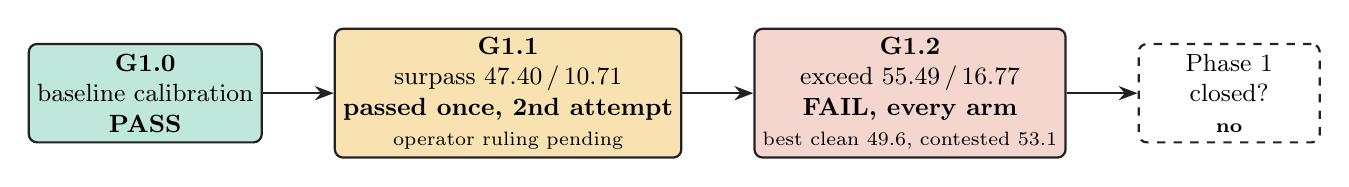
\begin{tikzpicture}[font=\small,
  box/.style={rectangle,rounded corners=3pt,draw=cLine,thick,minimum width=2.9cm,minimum height=1.25cm,align=center,inner sep=3pt},
  arr/.style={-{Stealth[length=2.4mm]},thick,cLine}]
  \node[box,fill=cGood!25] (g0) {\textbf{G1.0}\\baseline calibration\\\textbf{PASS}};
  \node[box,fill=cWarn!30,right=0.9cm of g0] (g1) {\textbf{G1.1}\\surpass 47.40\,/\,10.71\\\textbf{passed once, 2nd attempt}\\{\scriptsize operator ruling pending}};
  \node[box,fill=cBad!20,right=0.9cm of g1] (g2) {\textbf{G1.2}\\exceed 55.49\,/\,16.77\\\textbf{FAIL, every arm}\\{\scriptsize best clean 49.6, contested 53.1}};
  \node[box,dashed,right=0.9cm of g2,minimum width=2.3cm] (p) {Phase 1\\closed?\\{\scriptsize \textbf{no}}};
  \draw[arr] (g0)--(g1); \draw[arr] (g1)--(g2); \draw[arr] (g2)--(p);
\end{tikzpicture}
\caption{Gate status after both trials. A phase closes only when \emph{every} gate passes under EP-A (roadmap rule \p{phase\_advance}). G1.S (EP-B screening) was not run. }
\end{figure}

% Overview ladder ----------------------------------------------------------
\begin{figure}[H]\centering
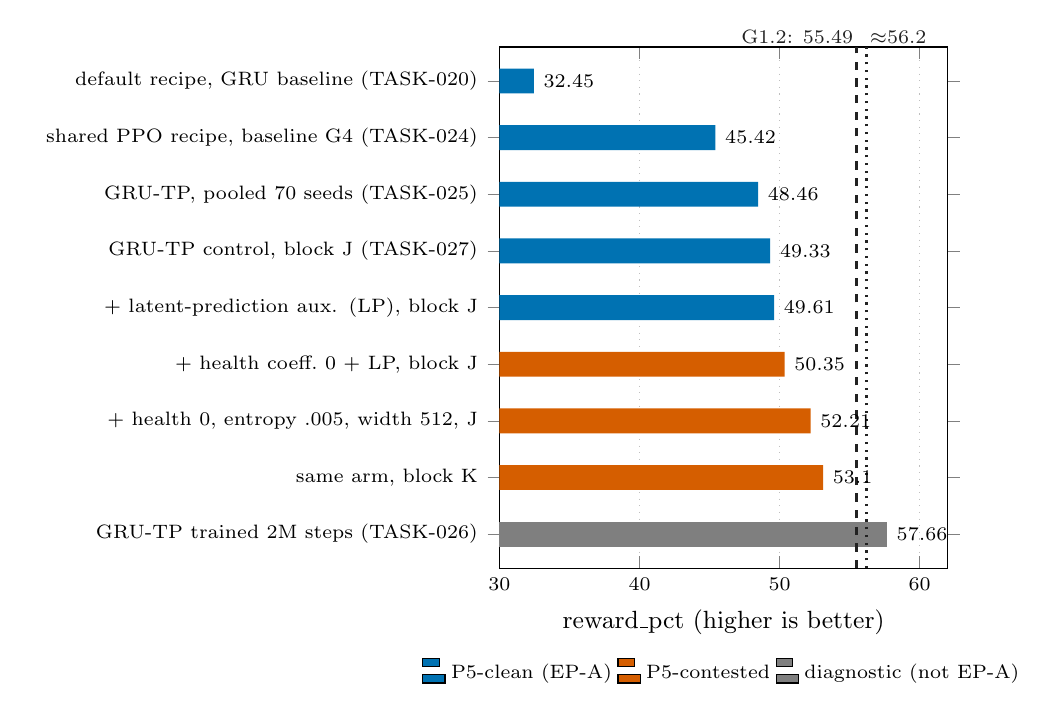
\begin{tikzpicture}
\begin{axis}[
  xbar, width=0.6\linewidth, height=8.2cm, bar width=9pt,
  xmin=30, xmax=62, xlabel={reward\_pct (higher is better)},
  y dir=reverse, ymin=0.4, ymax=9.6,
  ytick={1,...,9}, yticklabels={
    {\scriptsize default recipe, GRU baseline (TASK-020)},
    {\scriptsize shared PPO recipe, baseline G4 (TASK-024)},
    {\scriptsize GRU-TP, pooled 70 seeds (TASK-025)},
    {\scriptsize GRU-TP control, block J (TASK-027)},
    {\scriptsize + latent-prediction aux. (LP), block J},
    {\scriptsize + health coeff.\ 0 + LP, block J},
    {\scriptsize + health 0, entropy .005, width 512, J},
    {\scriptsize same arm, block K},
    {\scriptsize GRU-TP trained 2M steps (TASK-026)}},
  yticklabel style={align=right,text width=5.6cm},
  tick label style={font=\scriptsize}, label style={font=\small},
  xmajorgrids, grid style={dotted,gray!50},
  nodes near coords, nodes near coords align={horizontal}, every node near coord/.append style={font=\scriptsize},
  legend style={at={(0.5,-0.16)},anchor=north,legend columns=3,font=\scriptsize,draw=none},
  clip=false]
 \addplot[bar shift=0pt,fill=cClean,draw=none] coordinates {(32.45,1) (45.42,2) (48.46,3) (49.33,4) (49.61,5)};
 \addplot[bar shift=0pt,fill=cCont,draw=none]  coordinates {(50.35,6) (52.21,7) (53.10,8)};
 \addplot[bar shift=0pt,fill=cDiag,draw=none]  coordinates {(57.66,9)};
 \legend{P5-clean (EP-A),P5-contested,diagnostic (not EP-A)}
 \draw[dashed,thick,cLine] (rel axis cs:0.7966,0) -- (rel axis cs:0.7966,1);
 \node[font=\scriptsize,anchor=south east,text=cLine,inner sep=1pt] at (rel axis cs:0.7966,1.0) {G1.2: 55.49};
 \draw[dotted,thick,cLine] (rel axis cs:0.8188,0) -- (rel axis cs:0.8188,1);
 \node[font=\scriptsize,anchor=south west,text=cLine,inner sep=1pt] at (rel axis cs:0.8188,1.0) {$\approx$56.2};
\end{axis}
\end{tikzpicture}
\caption{How far each arm is from the G1.2 line. Dashed: the paper value 55.49. Dotted: the mean a low-variance arm needs so that mean $-$ 2\,SE exceeds 55.49 ($\approx56.2$, quoted from the TASK-026 report).
The 2M-step bar is a data-scaling diagnostic (2 seeds, different step budget), shown only to indicate where the gap closes. Values are the means reported for each row; spreads are in Section~\ref{sec:t027}.}
\label{fig:ladder}
\end{figure}

\paragraph{The two trials side by side.}
\begin{center}\small
\begin{tabular}{@{}p{2.6cm}p{6.7cm}p{6.7cm}@{}}\toprule
 & \textbf{TASK-026} (2026-10-19) & \textbf{TASK-027} (2026-10-22)\\\midrule
Question & Can ten single-knob changes of GRU-TP close the 7.7 reward gap? Where does the gap come from? & Can an lr schedule, a learned reward coefficient, or parameter changes raise sample efficiency toward G1.2?\\
Platform & cloud session, 4 CPU cores, jax 0.12.0 & Kaggle T4, jax 0.11.1 (screens and finals)\\
Seeds & tuning 4000--4003 (R0), 4000--4001 (variants) & tuning 4000--4003, 5000--5003, 6000--6003; finals 172--181 (J), 182--191 (K)\\
Final EP-A block? & none (pre-registered stop line 54.0 not reached) & yes: four arms in block J, one arm also in block K\\
Outcome & no knob qualifies; \textbf{2M steps crosses G1.2} $\Rightarrow$ gap is sample efficiency & clean arm $+0.28\pm0.60$ reward; contested best 52.21 / 53.10; \textbf{G1.2 fails}\\\bottomrule
\end{tabular}
\end{center}

% -------------------------------------------------------------------------------------------------
\section{Common setting and protocols}

\begin{center}\small
\begin{tabular}{@{}p{4.6cm}p{3.0cm}p{8.3cm}@{}}\toprule
\textbf{Label} & \textbf{Used for} & \textbf{Rules (abridged)}\\\midrule
\p{EP-A} & gate evidence & 999{,}424 env steps, 10 seeds (all listed), first episode of 256 fresh envs per seed, sampled policy, final checkpoint, clean commit, tuning on disjoint seeds\\
\p{EP-A-tuning} & screening & same budget and metrics, 2--4 seeds, tuning seeds only; never a gate\\
\p{diag-*} & diagnostics & other step budgets (2M/3M/4M); never a gate, never quoted beside paper numbers\\
\p{EP-A-P5-contested-\allowbreak reward-coefficient} & reward-coefficient arms & EP-A mechanics, but the \emph{training} reward is altered, which violates prohibition P5; MLflow \p{gate\_eligible=false}\\\bottomrule
\end{tabular}
\end{center}

\begin{center}\small
\begin{tabular}{@{}p{4.1cm}p{11.8cm}@{}}\toprule
\textbf{Reference arm} & \textbf{GRU-TP} (registry \p{Base\_O02\_D04\_S00}, config \p{G4TP1}): GRU baseline with LayerNorm and skip heads (G4), plus the transition-prediction (TP) auxiliary head. 1.254M params total, 0.880M deployed. It is the control in both trials.\\
\textbf{Thresholds (G1.2)} & MFRL\_best, Dedieu et al.\ 2025 Table~1: 55.49 reward, 16.77 score (55.6M params, image observation; modality caveat recorded). \\
\textbf{Starting point} & Best clean arm before these trials: GRU-TP pooled over 70 seeds $48.46\pm0.15$ reward, $18.51\pm0.21$ score. Score already clears 16.77; reward needs about $+7.7$ (about 1.6 more achievements per episode).\\\bottomrule
\end{tabular}
\end{center}

% -------------------------------------------------------------------------------------------------
\section{TASK-026: tuning attempt and data-scaling diagnostic}\label{sec:t026}

\subsection{Ten single-knob variants: none helps}
Pre-registered rule: a variant \emph{qualifies} if it beats R0 by $+2.0$ reward on the same seeds, and a final EP-A block is run only if some variant exceeds a 54.0 stop line.

\begin{figure}[H]\centering
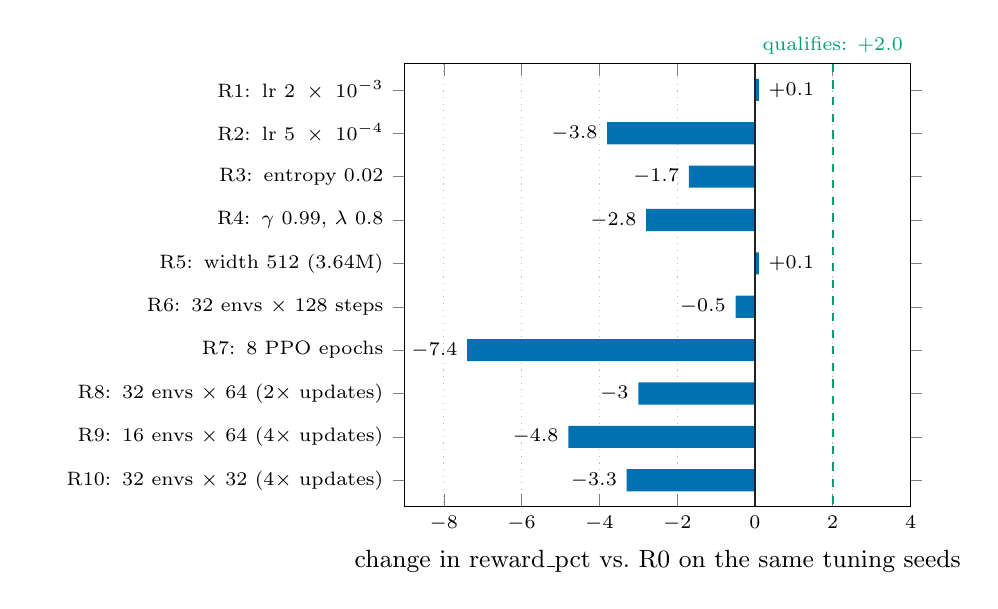
\begin{tikzpicture}
\begin{axis}[
  xbar, width=0.66\linewidth, height=7.2cm, bar width=8pt,
  xmin=-9, xmax=4, xlabel={change in reward\_pct vs.\ R0 on the same tuning seeds},
  y dir=reverse, ymin=0.4, ymax=10.6,
  ytick={1,...,10}, yticklabels={
    {\scriptsize R1: lr $2\!\times\!10^{-3}$},{\scriptsize R2: lr $5\!\times\!10^{-4}$},{\scriptsize R3: entropy 0.02},
    {\scriptsize R4: $\gamma$ 0.99, $\lambda$ 0.8},{\scriptsize R5: width 512 (3.64M)},{\scriptsize R6: 32 envs $\times$ 128 steps},
    {\scriptsize R7: 8 PPO epochs},{\scriptsize R8: 32 envs $\times$ 64 (2$\times$ updates)},{\scriptsize R9: 16 envs $\times$ 64 (4$\times$ updates)},
    {\scriptsize R10: 32 envs $\times$ 32 (4$\times$ updates)}},
  yticklabel style={align=right,text width=4.4cm},
  tick label style={font=\scriptsize}, label style={font=\small},
  xmajorgrids, grid style={dotted,gray!50},
  nodes near coords, every node near coord/.append style={font=\scriptsize,/pgf/number format/fixed,/pgf/number format/precision=1,/pgf/number format/showpos},
  nodes near coords align={horizontal}, clip=false]
 \addplot[bar shift=0pt,fill=cClean,draw=none] coordinates {(0.1,1) (-3.8,2) (-1.7,3) (-2.8,4) (0.1,5) (-0.5,6) (-7.4,7) (-3.0,8) (-4.8,9) (-3.3,10)};
 \draw[thick,cLine] (axis cs:0,0.4) -- (axis cs:0,10.6);
 \draw[dashed,thick,cGood] (axis cs:2,0.4) -- (axis cs:2,10.6);
 \node[font=\scriptsize,text=cGood,anchor=south] at (axis cs:2,0.4) {qualifies: $+2.0$};
\end{axis}
\end{tikzpicture}
\caption{TASK-026, one-factor screen around GRU-TP at the EP-A budget (differences as listed in the report, section~8.1; R0 $=48.83\pm0.45$ reward on 4 seeds, $48.62$ on the 2-seed subset used for most variants).
\textbf{Reading:} nothing reaches the green line; every variant that gives the PPO learner more updates per environment step (R7--R10) is \emph{worse}. By the pre-registered rule no final block was run.}
\label{fig:t026knobs}
\end{figure}

\subsection{Data-scaling diagnostic: the gap is sample efficiency}
The same GRU-TP configuration was trained for more environment steps (labelled \p{diag-*}, learning-rate schedule scaled to the run length, 2 seeds beyond 1M).

\begin{figure}[H]\centering
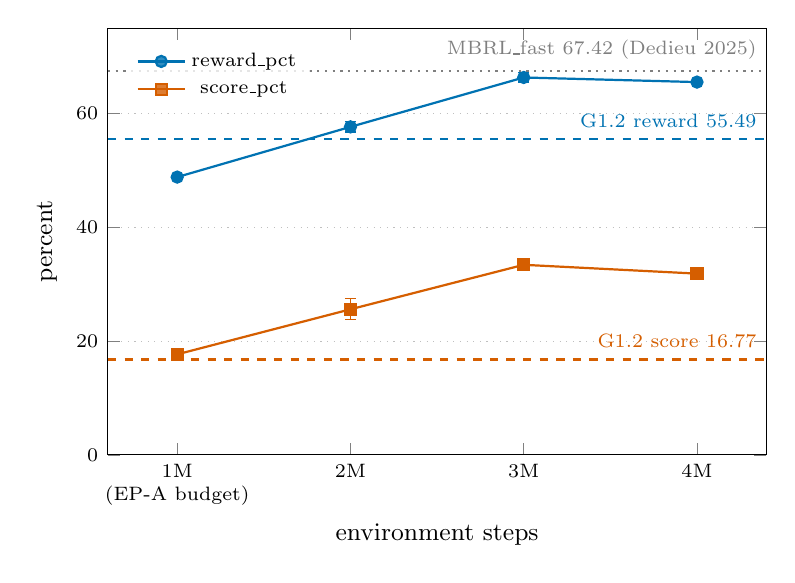
\begin{tikzpicture}
\begin{axis}[
  width=0.82\linewidth, height=7.0cm, xmin=0.6, xmax=4.4, ymin=0, ymax=75,
  xtick={1,2,3,4}, xticklabels={1M\\(EP-A budget),2M,3M,4M}, xticklabel style={align=center,font=\scriptsize},
  xlabel={environment steps}, ylabel={percent}, tick label style={font=\scriptsize}, label style={font=\small},
  ymajorgrids, grid style={dotted,gray!50},
  legend style={at={(0.03,0.97)},anchor=north west,font=\scriptsize,draw=none,fill=white,fill opacity=0.8,text opacity=1},
  error bars/y dir=both, error bars/y explicit]
 \addplot[thick,cClean,mark=*,error bars/.cd,y dir=both,y explicit] coordinates {(1,48.83) +- (0,0.45) (2,57.66) +- (0,0.90) (3,66.34) +- (0,0.80) (4,65.53) +- (0,0.15)};
 \addlegendentry{reward\_pct}
 \addplot[thick,cCont,mark=square*,error bars/.cd,y dir=both,y explicit] coordinates {(1,17.67) +- (0,0.67) (2,25.59) +- (0,1.84) (3,33.41) +- (0,0.30) (4,31.86) +- (0,0.24)};
 \addlegendentry{score\_pct}
 \addplot[dashed,thick,cClean,no marks,forget plot] coordinates {(0.6,55.49) (4.4,55.49)};
 \node[font=\scriptsize,text=cClean,anchor=south east] at (axis cs:4.4,55.9) {G1.2 reward 55.49};
 \addplot[dashed,thick,cCont,no marks,forget plot] coordinates {(0.6,16.77) (4.4,16.77)};
 \node[font=\scriptsize,text=cCont,anchor=south east] at (axis cs:4.4,17.2) {G1.2 score 16.77};
 \addplot[dotted,thick,cDiag,no marks,forget plot] coordinates {(0.6,67.42) (4.4,67.42)};
 \node[font=\scriptsize,text=cDiag,anchor=south east] at (axis cs:4.4,67.8) {MBRL\_fast 67.42 (Dedieu 2025)};
\end{axis}
\end{tikzpicture}
\caption{TASK-026 data-scaling diagnostic (mean $\pm$ SE; 1M: 4 seeds, others: 2 seeds, single configuration, CPU). \textbf{Reading:} the curve crosses both G1.2 lines between 1M and 2M steps
(2M: reward $-2$\,SE $=55.87$) and plateaus near 66 reward from 3M. This is why the report concludes that the missing quantity is learning per environment step (about $1.7$--$2\times$), not model capacity.
The shape, not the exact values, is the finding.}
\label{fig:scaling}
\end{figure}

\begin{figure}[H]\centering
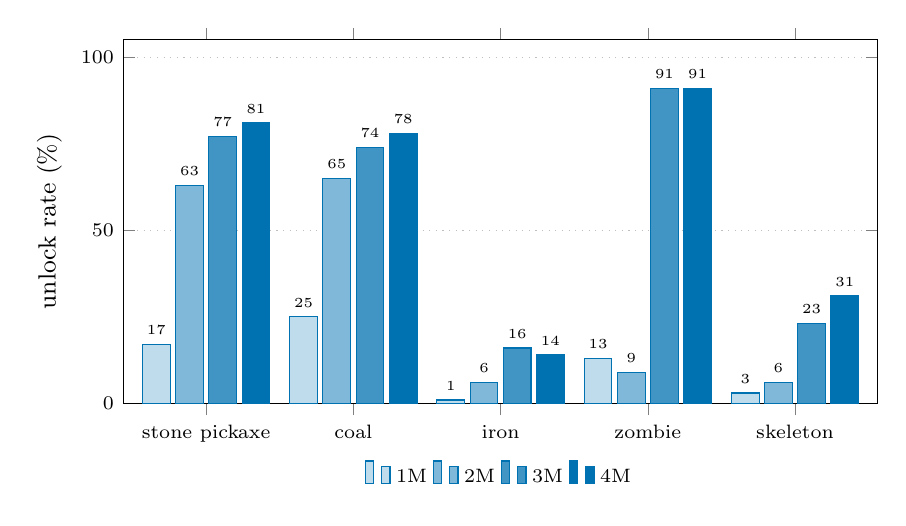
\begin{tikzpicture}
\begin{axis}[
  ybar, width=0.92\linewidth, height=6.2cm, bar width=10pt, ymin=0, ymax=105,
  symbolic x coords={stone pickaxe,coal,iron,zombie,skeleton}, xtick=data, enlarge x limits=0.14,
  ylabel={unlock rate (\%)}, tick label style={font=\scriptsize}, label style={font=\small},
  ymajorgrids, grid style={dotted,gray!50},
  legend style={at={(0.5,-0.14)},anchor=north,legend columns=4,font=\scriptsize,draw=none},
  nodes near coords, every node near coord/.append style={font=\tiny}]
 \addplot[fill=cClean!25,draw=cClean] coordinates {(stone pickaxe,17) (coal,25) (iron,1) (zombie,13) (skeleton,3)};
 \addplot[fill=cClean!50,draw=cClean] coordinates {(stone pickaxe,63) (coal,65) (iron,6) (zombie,9) (skeleton,6)};
 \addplot[fill=cClean!75,draw=cClean] coordinates {(stone pickaxe,77) (coal,74) (iron,16) (zombie,91) (skeleton,23)};
 \addplot[fill=cClean,draw=cClean] coordinates {(stone pickaxe,81) (coal,78) (iron,14) (zombie,91) (skeleton,31)};
 \legend{1M,2M,3M,4M}
\end{axis}
\end{tikzpicture}
\caption{TASK-026, unlock rates of the deep achievement chain for GRU-TP at 1M, 2M, 3M, 4M steps (report section~8.2). \textbf{Reading:} the 1M policy is stuck at the start of the tech chain
(iron $\approx1\%$); the extra data is spent on stone tools, coal, then iron and the monsters. \p{eat\_plant}, diamond and iron tools remain at $0\%$ even at 4M (not drawn).}
\label{fig:ach}
\end{figure}

\subsection{Ceiling argument (1M-step policies only)}
Taking, for every achievement, the best unlock rate over the five 1M-step arms of TASK-025 gives a union of \textbf{52.63} reward ($11.58$ achievements per episode), still below 55.49 ($12.21$ per episode).
The arms are complementary (GRU-TP raises \p{eat\_cow} 45$\to$75\,\%, Truck variants defeat zombies 47--59\,\% vs.\ 10--16\,\%), but no mix of 1M-step policies reaches the gate.
This is a statement about the EP-A budget, not about what the model family can represent (Fig.~\ref{fig:ach}).

\subsection{Conclusions of TASK-026}
\begin{itemize}\itemsep1pt
\item \textbf{Knob tuning is exhausted for G1.2} at 1M steps: ten single-knob variants, none above $+0.1$ reward.
\item \textbf{The first-draft reading was corrected}: the pre-registration expected a missing capability; the diagnostic shows a sample-efficiency gap (README amendment 4).
\item \textbf{No final block, no gate claim.} Candidate directions (none implemented, since each is an unconfirmed component): Dyna-style use of the TP head, an off-policy/high update-to-data learner, more TP-like auxiliary signals, image modality.
\end{itemize}

% -------------------------------------------------------------------------------------------------
\section{TASK-027: sample-efficiency ideas for G1.2}\label{sec:t027}

\subsection{Design: three operator ideas and one addition}
\begin{figure}[H]\centering
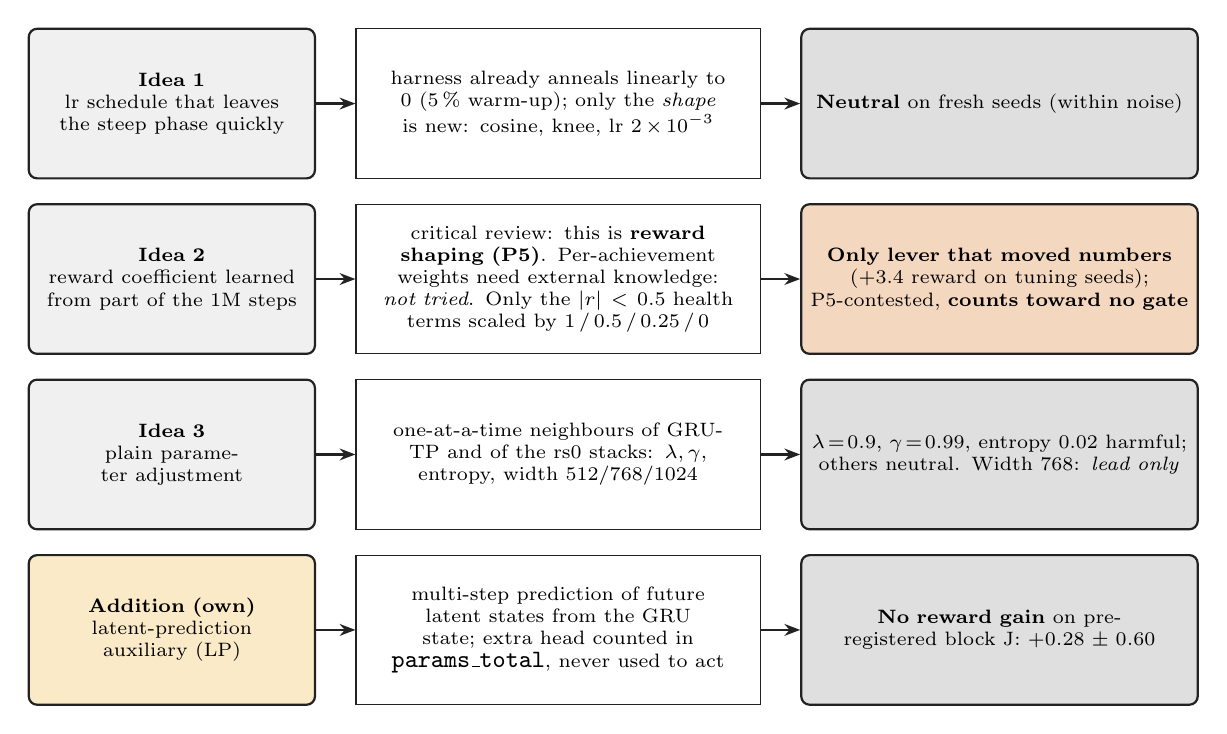
\begin{tikzpicture}[font=\scriptsize,
  idea/.style={rectangle,rounded corners=3pt,draw=cLine,thick,fill=#1,minimum width=3.5cm,minimum height=1.9cm,align=center,text width=3.4cm},
  res/.style={rectangle,rounded corners=3pt,draw=cLine,thick,fill=#1,minimum width=4.9cm,minimum height=1.9cm,align=center,text width=4.8cm},
  mid/.style={rectangle,draw=cLine,thin,fill=white,minimum width=5.0cm,minimum height=1.9cm,align=center,text width=4.9cm},
  arr/.style={-{Stealth[length=2mm]},thick,cLine}]
  \node[idea=gray!12] (i1) {\textbf{Idea 1}\\lr schedule that leaves the steep phase quickly};
  \node[idea=gray!12,below=0.3cm of i1] (i2) {\textbf{Idea 2}\\reward coefficient learned from part of the 1M steps};
  \node[idea=gray!12,below=0.3cm of i2] (i3) {\textbf{Idea 3}\\plain parameter adjustment};
  \node[idea=cWarn!22,below=0.3cm of i3] (i4) {\textbf{Addition (own)}\\latent-prediction auxiliary (LP)};
  \node[mid,right=0.5cm of i1] (m1) {harness already anneals linearly to 0 (5\,\% warm-up); only the \emph{shape} is new: cosine, knee, lr $2\!\times\!10^{-3}$};
  \node[mid,right=0.5cm of i2] (m2) {critical review: this is \textbf{reward shaping (P5)}. Per-achievement weights need external knowledge: \emph{not tried}. Only the $|r|<0.5$ health terms scaled by 1\,/\,0.5\,/\,0.25\,/\,0};
  \node[mid,right=0.5cm of i3] (m3) {one-at-a-time neighbours of GRU-TP and of the rs0 stacks: $\lambda,\gamma$, entropy, width 512/768/1024};
  \node[mid,right=0.5cm of i4] (m4) {multi-step prediction of future latent states from the GRU state; extra head counted in \p{params\_total}, never used to act};
  \node[res=cDiag!25,right=0.5cm of m1] (r1) {\textbf{Neutral} on fresh seeds (within noise)};
  \node[res=cCont!25,right=0.5cm of m2] (r2) {\textbf{Only lever that moved numbers} (+3.4 reward on tuning seeds); P5-contested, \textbf{counts toward no gate}};
  \node[res=cDiag!25,right=0.5cm of m3] (r3) {$\lambda\!=\!0.9$, $\gamma\!=\!0.99$, entropy 0.02 harmful; others neutral. Width 768: \emph{lead only}};
  \node[res=cDiag!25,right=0.5cm of m4] (r4) {\textbf{No reward gain} on pre-registered block J: $+0.28\pm0.60$};
  \foreach \a/\b in {i1/m1,i2/m2,i3/m3,i4/m4,m1/r1,m2/r2,m3/r3,m4/r4} \draw[arr] (\a)--(\b);
\end{tikzpicture}
\caption{TASK-027 design and outcome, one row per idea. Idea~1 is the operator's wording; the coefficient in idea~2 was \emph{not learned}: the effect is monotone and ends at 0, so a learned
coefficient would have to converge to ``ignore the health reward'', and no principled criterion for that exists that does not already encode that the metric counts achievements.}
\label{fig:design}
\end{figure}

\subsection{Screening on tuning seeds: one round in detail}
\begin{figure}[H]\centering
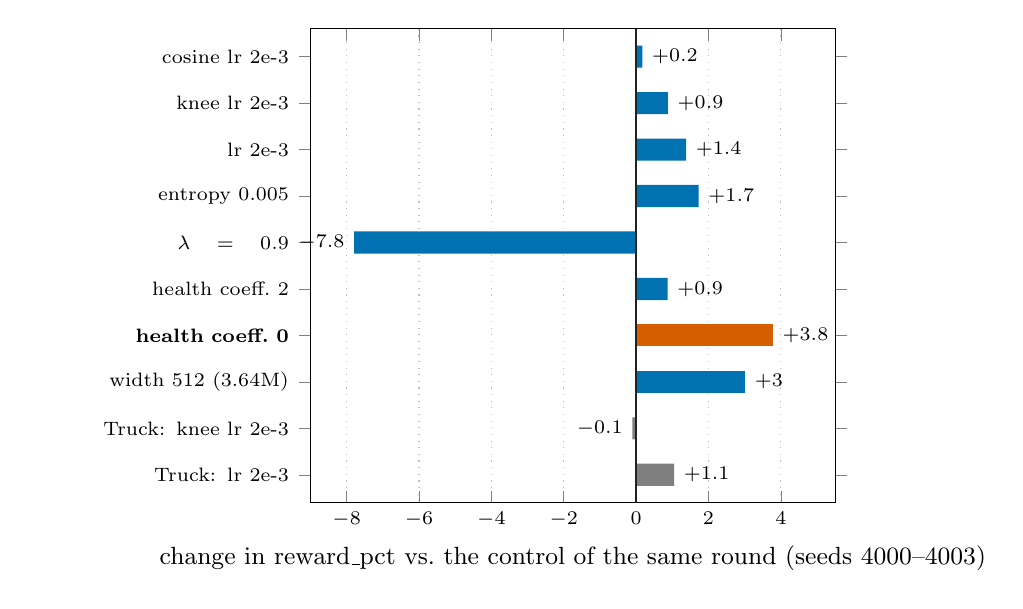
\begin{tikzpicture}
\begin{axis}[
  xbar, width=0.68\linewidth, height=7.6cm, bar width=8pt,
  xmin=-9, xmax=5.5, xlabel={change in reward\_pct vs.\ the control of the same round (seeds 4000--4003)},
  y dir=reverse, ymin=0.4, ymax=10.6,
  ytick={1,...,10}, yticklabels={
    {\scriptsize cosine lr 2e-3},{\scriptsize knee lr 2e-3},{\scriptsize lr 2e-3},{\scriptsize entropy 0.005},{\scriptsize $\lambda=0.9$},
    {\scriptsize health coeff.\ 2},{\scriptsize \textbf{health coeff.\ 0}},{\scriptsize width 512 (3.64M)},
    {\scriptsize Truck: knee lr 2e-3},{\scriptsize Truck: lr 2e-3}},
  yticklabel style={align=right,text width=3.2cm},
  tick label style={font=\scriptsize}, label style={font=\small},
  xmajorgrids, grid style={dotted,gray!50},
  nodes near coords, every node near coord/.append style={font=\scriptsize,/pgf/number format/fixed,/pgf/number format/precision=1,/pgf/number format/showpos},
  nodes near coords align={horizontal}, clip=false]
 \addplot[bar shift=0pt,fill=cClean,draw=none] coordinates {(0.17,1) (0.88,2) (1.38,3) (1.73,4) (-7.79,5) (0.87,6)};
 \addplot[bar shift=0pt,fill=cCont,draw=none]  coordinates {(3.78,7)};
 \addplot[bar shift=0pt,fill=cClean,draw=none] coordinates {(3.01,8)};
 \addplot[bar shift=0pt,fill=cDiag,draw=none]  coordinates {(-0.10,9) (1.05,10)};
 \draw[thick,cLine] (axis cs:0,0.4) -- (axis cs:0,10.6);
\end{axis}
\end{tikzpicture}
\caption{TASK-027 round R1 (4 seeds each; differences computed from Appendix~\ref{app:screens}: GRU rows against \p{G4TP1} $=47.11$, Truck rows against the Truck-plus-TP-head control \p{TP1h} $=45.94$).
\textbf{Reading:} only the health coefficient 0 and width 512 stand out. Please note the noise floor: the identical configuration and seeds gave $48.83$ in TASK-026 (CPU) and $47.11$ here (T4), a $1.7$ difference, so differences below about $2$ are not interpretable. }
\label{fig:r1}
\end{figure}

\subsection{The reward-coefficient lever: monotone, but it is reward shaping}
\begin{figure}[H]\centering
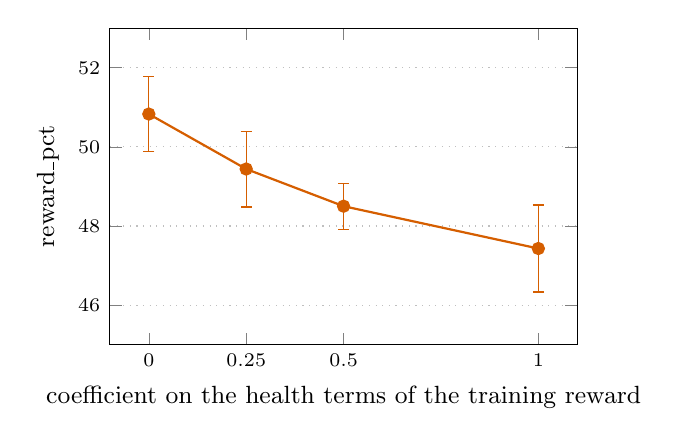
\begin{tikzpicture}
\begin{axis}[
  width=0.62\linewidth, height=5.6cm, xmin=-0.1, xmax=1.1, ymin=45, ymax=53,
  xtick={0,0.25,0.5,1}, xlabel={coefficient on the health terms of the training reward}, ylabel={reward\_pct},
  tick label style={font=\scriptsize}, label style={font=\small}, ymajorgrids, grid style={dotted,gray!50}]
 \addplot[thick,cCont,mark=*,error bars/.cd,y dir=both,y explicit] coordinates {(0,50.83) +- (0,0.94) (0.25,49.44) +- (0,0.96) (0.5,48.50) +- (0,0.58) (1,47.43) +- (0,1.10)};
\end{axis}
\end{tikzpicture}
\caption{Dose-response of the health-term coefficient (rounds R2--R4, seeds 5000--5003, GRU-TP; mean $\pm$ SE). The coefficient $1$ point is the unmodified control \p{G4TP1}.
\textbf{Reading:} a clean monotone trend ($47.4\to50.8$), reproduced on a second seed set (4000--4003: $47.11\to50.89$ at coefficient $1\to0$). Because the effect ends at 0, it is ``ignore health reward'': a protocol-level change, not a learning gain.}
\label{fig:dose}
\end{figure}

\subsection{Screening gains shrink on fresh seeds (winner's curse)}
\begin{figure}[H]\centering
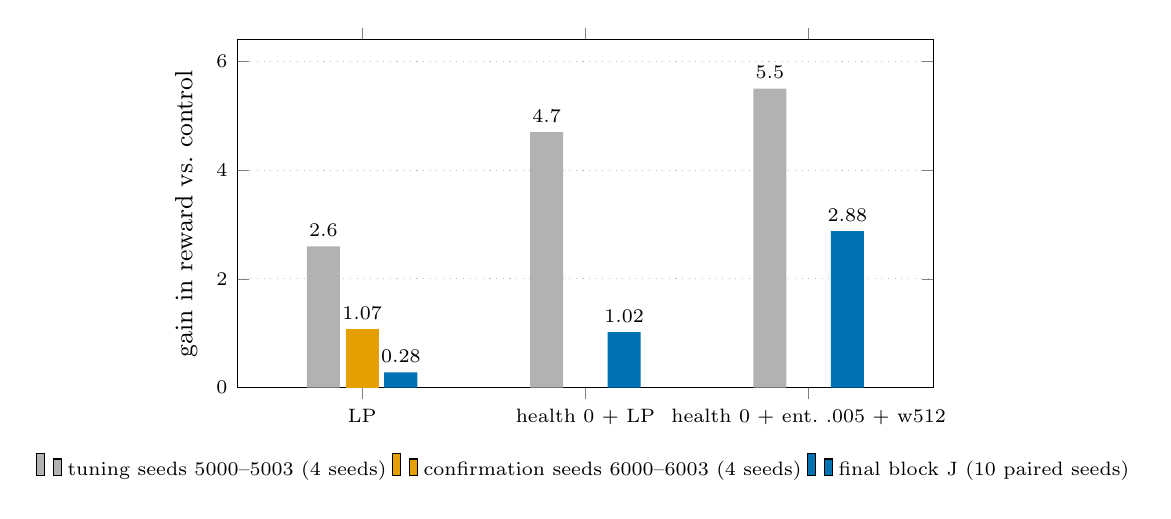
\begin{tikzpicture}
\begin{axis}[
  ybar, width=0.86\linewidth, height=6.0cm, bar width=12pt, ymin=0, ymax=6.4,
  symbolic x coords={LP,{health 0 + LP},{health 0 + ent.\ .005 + w512}}, xtick=data, enlarge x limits=0.28,
  ylabel={gain in reward vs.\ control}, tick label style={font=\scriptsize}, label style={font=\small},
  ymajorgrids, grid style={dotted,gray!50},
  legend style={at={(0.5,-0.17)},anchor=north,legend columns=3,font=\scriptsize,draw=none},
  nodes near coords, every node near coord/.append style={font=\scriptsize,/pgf/number format/fixed,/pgf/number format/precision=2}]
 \addplot[fill=cDiag!60,draw=none] coordinates {(LP,2.60) ({health 0 + LP},4.70) ({health 0 + ent.\ .005 + w512},5.50)};
 \addplot[fill=cWarn,draw=none]    coordinates {(LP,1.07)};
 \addplot[fill=cClean,draw=none]   coordinates {(LP,0.28) ({health 0 + LP},1.02) ({health 0 + ent.\ .005 + w512},2.88)};
 \legend{tuning seeds 5000--5003 (4 seeds),confirmation seeds 6000--6003 (4 seeds),final block J (10 paired seeds)}
\end{axis}
\end{tikzpicture}
\caption{Gain over the GRU-TP control in the screening round versus the pre-registered final block. Tuning and confirmation gains are differences of 4-seed means (Appendix~\ref{app:screens}); final gains are paired
differences over 10 seeds (RESULTS section~5). \textbf{Reading:} every gain shrinks on fresh seeds, which is the expected behaviour of selecting the best of about 35 configurations. The LP gain falls from $+2.60$ to $+0.28\pm0.60$ (not distinguishable from zero).}
\label{fig:curse}
\end{figure}

\subsection{Final EP-A blocks}
\begin{figure}[H]\centering
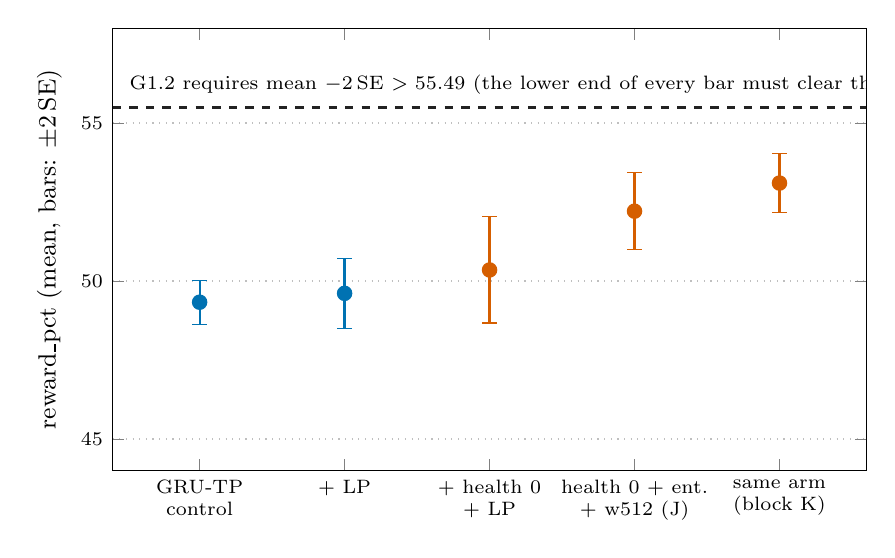
\begin{tikzpicture}
\begin{axis}[
  width=0.92\linewidth, height=7.2cm, xmin=0.4, xmax=5.6, ymin=44, ymax=58,
  xtick={1,2,3,4,5}, xticklabels={GRU-TP\\control,+ LP,+ health 0\\+ LP,health 0 + ent.\\+ w512 (J),same arm\\(block K)},
  xticklabel style={align=center,font=\scriptsize},
  ylabel={reward\_pct (mean, bars: $\pm2$\,SE)}, tick label style={font=\scriptsize}, label style={font=\small},
  ymajorgrids, grid style={dotted,gray!50}]
 \addplot[only marks,mark=*,mark size=2.6pt,cClean,error bars/.cd,y dir=both,y explicit,error bar style={thick}] coordinates {(1,49.33) +- (0,0.70) (2,49.61) +- (0,1.10)};
 \addplot[only marks,mark=*,mark size=2.6pt,cCont,error bars/.cd,y dir=both,y explicit,error bar style={thick}] coordinates {(3,50.35) +- (0,1.68) (4,52.21) +- (0,1.22) (5,53.10) +- (0,0.94)};
 \draw[dashed,thick,cLine] (axis cs:0.4,55.49) -- (axis cs:5.6,55.49);
 \node[font=\scriptsize,anchor=south west] at (axis cs:0.45,55.6) {G1.2 requires mean $-2$\,SE $>55.49$ (the lower end of every bar must clear this line)};
\end{axis}
\end{tikzpicture}
\caption{Final blocks, 10 seeds each: mean with a $\pm2$\,SE bar. Blue: P5-clean. Orange: P5-contested. \textbf{Reading:} no lower bar end comes within $3.3$ reward of the dashed line.
Blocks J and K for the last arm are independent seed sets (train 172--181 / test 554--563, and train 182--191 / test 564--573).}
\label{fig:final}
\end{figure}

\begin{center}\small
\begin{tabular}{@{}p{3.6cm}lrcccccc@{}}\toprule
arm & protocol & params & reward (mean $\pm$ SE) & $-$2SE & score (mean $\pm$ SE) & $-$2SE & G1.2 & gap\textsuperscript{a}\\\midrule
\p{G4TP1} (control, J) & EP-A & 1.25M & $49.33\pm0.35$ & 48.62 & $19.01\pm0.46$ & 18.09 & fail & 6.87\\
\p{G\_lp1} (J) & EP-A & 1.52M & $49.61\pm0.55$ & 48.52 & $19.88\pm0.41$ & 19.06 & fail & 6.97\\
\p{G\_rs0\_lp1} (J) & contested & 1.52M & $50.35\pm0.84$ & 48.66 & $20.28\pm0.65$ & 18.99 & fail & 6.83\\
\p{G\_rs0\_ent005\_w512} (J) & contested & 3.64M & $52.21\pm0.61$ & 50.98 & $20.32\pm0.78$ & 18.76 & fail & 4.51\\
\p{G\_rs0\_ent005\_w512} (K) & contested & 3.64M & $53.10\pm0.47$ & 52.16 & $21.86\pm0.52$ & 20.82 & fail & 3.33\\\bottomrule
\end{tabular}\\[2pt]
{\scriptsize \textsuperscript{a}\,gap $=55.49-(\text{mean}-2\,\text{SE})$ on reward (arithmetic on the table values). Score clears 16.77 for every arm; reward is the only failing metric.}
\end{center}

\noindent\textbf{Paired differences to the same-seed control} (block J, $n=10$; seed $s$ uses test seed $s+382$ for every arm).\par\nopagebreak\medskip
\begin{figure}[H]\centering
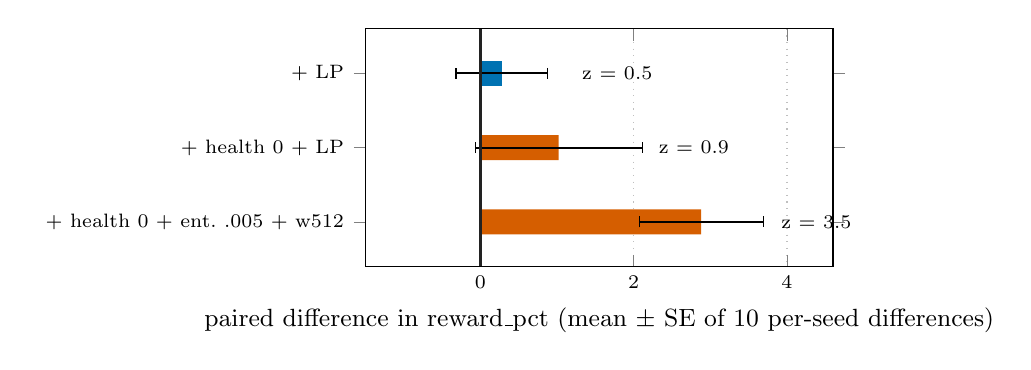
\begin{tikzpicture}
\begin{axis}[
  xbar, width=0.62\linewidth, height=4.6cm, bar width=9pt, xmin=-1.5, xmax=4.6,
  y dir=reverse, ymin=0.4, ymax=3.6, ytick={1,2,3}, yticklabels={{\scriptsize + LP},{\scriptsize + health 0 + LP},{\scriptsize + health 0 + ent.\ .005 + w512}},
  yticklabel style={align=right,text width=3.9cm}, xlabel={paired difference in reward\_pct (mean $\pm$ SE of 10 per-seed differences)},
  tick label style={font=\scriptsize}, label style={font=\small}, xmajorgrids, grid style={dotted,gray!50}, clip=false]
 \addplot[bar shift=0pt,fill=cClean,draw=none,error bars/.cd,x dir=both,x explicit,error bar style={thick}] coordinates {(0.28,1) +- (0.60,0)};
 \addplot[bar shift=0pt,fill=cCont,draw=none,error bars/.cd,x dir=both,x explicit,error bar style={thick}] coordinates {(1.02,2) +- (1.09,0) (2.88,3) +- (0.81,0)};
 \draw[thick,cLine] (axis cs:0,0.4) -- (axis cs:0,3.6);
 \node[font=\scriptsize,anchor=west] at (axis cs:1.2,1) {z = 0.5};
 \node[font=\scriptsize,anchor=west] at (axis cs:2.2,2) {z = 0.9};
 \node[font=\scriptsize,anchor=west] at (axis cs:3.8,3) {z = 3.5};
\end{axis}
\end{tikzpicture}
\caption{Paired reward differences in block J (RESULTS section~5). Score differences: $+0.86\pm0.38$ (z 2.3), $+1.27\pm0.96$ (z 1.3), $+1.31\pm1.07$ (z 1.2).
\textbf{Reading:} LP is indistinguishable from the control on reward; only the full contested stack shows a reward gain clearly above noise ($+2.88\pm0.81$), and it is the one that violates P5.}
\label{fig:paired}
\end{figure}

\subsection{Width round: a lead, not a result}
\begin{figure}[H]\centering
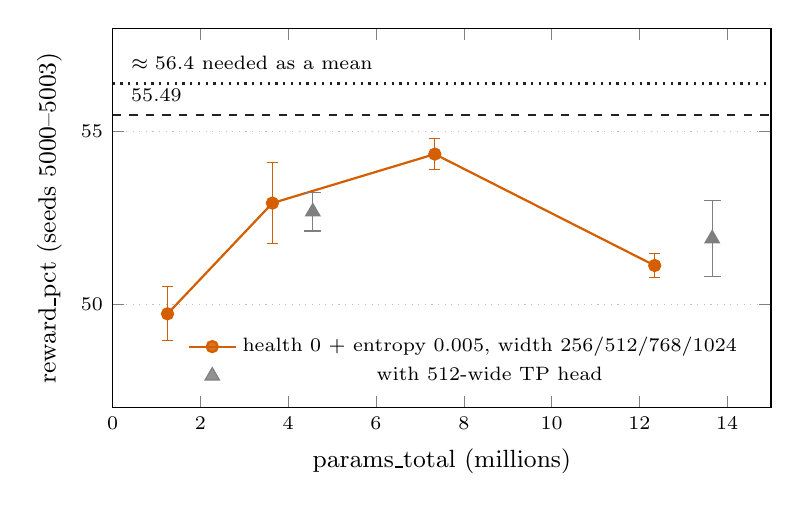
\begin{tikzpicture}
\begin{axis}[
  width=0.82\linewidth, height=6.4cm, xmin=0, xmax=15, ymin=47, ymax=58, xlabel={params\_total (millions)}, ylabel={reward\_pct (seeds 5000--5003)},
  tick label style={font=\scriptsize}, label style={font=\small}, ymajorgrids, grid style={dotted,gray!50},
  legend style={at={(0.97,0.03)},anchor=south east,font=\scriptsize,fill=white,fill opacity=0.85,text opacity=1,draw=none}]
 \addplot[thick,cCont,mark=*,error bars/.cd,y dir=both,y explicit] coordinates {(1.25,49.72) +- (0,0.78) (3.64,52.93) +- (0,1.18) (7.34,54.35) +- (0,0.45) (12.35,51.12) +- (0,0.34)};
 \addlegendentry{health 0 + entropy 0.005, width 256/512/768/1024}
 \addplot[only marks,mark=triangle*,mark size=3pt,cDiag,error bars/.cd,y dir=both,y explicit] coordinates {(4.56,52.68) +- (0,0.56) (13.66,51.90) +- (0,1.11)};
 \addlegendentry{with 512-wide TP head}
 \addplot[dashed,thick,cLine,no marks,forget plot] coordinates {(0,55.49) (15,55.49)};
 \node[font=\scriptsize,anchor=south west] at (axis cs:0.2,55.6) {55.49};
 \addplot[dotted,thick,cLine,no marks,forget plot] coordinates {(0,56.4) (15,56.4)};
 \node[font=\scriptsize,anchor=south west] at (axis cs:0.2,56.5) {$\approx56.4$ needed as a mean};
\end{axis}
\end{tikzpicture}
\caption{Round R7: width and TP-head size, all P5-contested, tuning seeds, $n=4$ (mean $\pm$ SE). Width 768 reached $54.35\pm0.45$ reward / $23.75\pm0.11$ score, the highest tuning-seed number of the task, but the response is non-monotone
(512: 52.93, 768: 54.35, 1024: 51.12), it is the best of four configurations screened on the same four seeds, and width 512 had already shrunk on fresh seeds. \textbf{No final block was run} (about 70 minutes of one kernel slot remained before the deadline), so width 768 is not gate evidence and, even if it held, would still need about $+2$ reward.}
\label{fig:width}
\end{figure}

\subsection{Conclusions of TASK-027}
\begin{itemize}\itemsep1pt
\item \textbf{G1.2 is not reached.} Best clean arm: $49.61$ (block J). Best contested arm: $52.21$ (J) and $53.10$ (K); $55.49$ needed at mean $-2$\,SE.
\item \textbf{No P5-clean lever moved reward}: lr shape, lr $2\!\times\!10^{-3}$, $\lambda$, $\gamma$, entropy, width and the new LP auxiliary were neutral or harmful on fresh seeds. TASK-026 found the same for the plain knobs.
\item \textbf{The one lever that moved numbers is reward shaping} (idea~2). It carries the labels \p{EP-A-P5-contested-\allowbreak reward-coefficient}, \p{gate\_eligible=false} and separate \p{+rs0} arm labels in MLflow.
\item \textbf{Distance remaining:} about $1.7\times$ data efficiency (TASK-026 2M-step diagnostic $57.7$); the best contested arm closes roughly $+3$ of the $\approx+9$ that doubling the data gives (no efficiency factor is claimed from this).
\end{itemize}

% -------------------------------------------------------------------------------------------------
\section{What the two trials establish}\label{sec:claims}
\small
\begin{longtable}{@{}p{5.9cm}p{4.1cm}p{5.6cm}@{}}\toprule
\textbf{Claim} & \textbf{Evidence} & \textbf{Strength and limits}\\\midrule\endhead
Plain PPO knobs (lr, entropy, $\gamma/\lambda$, epochs, batch shape, width) do not close G1.2 & TASK-026 (10 variants, 2--4 seeds); TASK-027 (about 35 configurations, 4 seeds) & Strong for ``no large effect''; screens detect only effects at least about 2 reward\\
More PPO updates per env step hurt & TASK-026 R7--R10 ($-3.0$ to $-7.4$) & Consistent in four variants; one config\\
The gap is sample efficiency, not capacity & TASK-026 2M/3M/4M diagnostic (Fig.~\ref{fig:scaling}); width 512--1024 gives no clean gain & Moderate: 2 seeds, one configuration, CPU; shape not exact values\\
The LP auxiliary does not raise reward & block J, paired $n=10$: $+0.28\pm0.60$ & Strong (pre-registered, fresh seeds); score $+0.86\pm0.38$ is suggestive only\\
Zeroing the health reward raises reward by about 1--3 & tuning seeds ($+3.4$), block J stack ($+2.88\pm0.81$) & Real but P5-contested; no gate value; smaller on fresh seeds\\
Width 768 might reach about 54 & one 4-seed tuning set & \textbf{Lead only}: best of four, non-monotone, no final block\\
A \emph{learned} reward coefficient & not built & Effect is monotone to 0, so no learning criterion was found that is not circular\\
Dyna-style imagination, off-policy high-UTD learner, image modality & not tested in either trial & Open; each needs a design decision\\\bottomrule
\end{longtable}
\normalsize

% -------------------------------------------------------------------------------------------------
\section{Caveats recorded in the task files}
\small
\begin{center}\begin{tabular}{@{}p{4.3cm}p{11.5cm}@{}}\toprule
\textbf{Caveat} & \textbf{Detail}\\\midrule
Seed overlap & Tuning seeds 4000--4003 are shared by TASK-026 and TASK-027; they were never used for a gate.\\
Unequal tuning effort (P9) & The tuned arms have about 35 configurations $\times$ 4 seeds of screening; the control has none (TASK-025 configuration). This favours the tuned arms.\\
Winner's curse & Screening gains shrink on fresh seeds (Fig.~\ref{fig:curse}); 2--4-seed means are optimistic by several points.\\
Not bit-reproducible & GPU runs differ run to run; across platforms the same configuration differed by $1.7$ reward (Fig.~\ref{fig:r1}).\\
Platforms differ & TASK-026 on a 4-core CPU (jax 0.12.0); TASK-027 on Kaggle T4 (jax 0.11.1). Within a block every arm ran on the same platform.\\
Modality & Our runs use the 1345-d symbolic observation; the paper thresholds use the 63$\times$63$\times$3 image, so calibration against them is approximate.\\
Diagnostics & The 2M--4M runs use 2 seeds and one configuration; they are \p{diag-*}, never a gate.\\
Open operator decisions & (a) Is any reward-coefficient arm admissible, i.e.\ amend P5? (b) Does GRU-TP's second-attempt G1.1 pass close G1.1?\\\bottomrule
\end{tabular}\end{center}
\normalsize

\section{Decisions we would kindly ask you to take}
\begin{enumerate}\itemsep2pt
\item \textbf{P5.} Keep the rule (the reward-coefficient arms stay diagnostics) or amend it, in which case the coefficient must be declared and the baseline given equal effort in a fresh pre-registered block.
\item \textbf{G1.1 ruling.} Whether GRU-TP's pass on its second attempt closes G1.1 (the roadmap defines no retry rule; all blocks are reported, none dropped).
\item \textbf{Next direction for sample efficiency.} Candidates, none built: Dyna-style use of the TP head (supported by TP being the only auxiliary that helped, and by Dedieu et al.\ reaching 67.4 at 1M steps with a transformer world model), an off-policy/high update-to-data learner (PPO with more reuse hurt), further TP-like auxiliary signals (the contrastive EV auxiliary hurt, so the choice matters), image modality. Each requires a design decision and a GPU.
\end{enumerate}

\appendix
\section{Complete screening tables of TASK-027}\label{app:screens}
\small
\begin{longtable}{@{}llrrrrr@{}}
\caption{All screening results of TASK-027 (Kaggle T4, 4 seeds per row; copied mechanically from \texttt{RESULTS.md}, sections 3--4). Reward and score are mean $\pm$ SE; r+s is their sum.}\label{tab:screens}\\
\toprule round & config & params\_total & reward & score & r+s & per-seed reward\\\midrule\endfirsthead
\toprule round & config & params\_total & reward & score & r+s & per-seed reward\\\midrule\endhead
\textbf{R1}\,{\scriptsize(seeds 4000-4003)} & \texttt{\scriptsize G4TP1} & 1,254,358 & 47.11 $\pm$ 0.79 & 17.39 $\pm$ 1.03 & 64.5 & {\scriptsize 48.7 48.2 46.2 45.4}\\
 & \texttt{\scriptsize G\_cos2} & 1,254,358 & 47.28 $\pm$ 0.46 & 16.15 $\pm$ 0.38 & 63.4 & {\scriptsize 47.2 46.5 48.6 46.8}\\
 & \texttt{\scriptsize G\_ent005} & 1,254,358 & 48.84 $\pm$ 0.61 & 18.81 $\pm$ 1.28 & 67.7 & {\scriptsize 49.7 48.3 47.4 50.0}\\
 & \texttt{\scriptsize G\_kn2a} & 1,254,358 & 47.99 $\pm$ 0.94 & 18.99 $\pm$ 0.91 & 67.0 & {\scriptsize 46.2 48.2 50.6 47.0}\\
 & \texttt{\scriptsize G\_lam9} & 1,254,358 & 39.32 $\pm$ 0.70 & 12.80 $\pm$ 0.50 & 52.1 & {\scriptsize 38.0 40.9 38.3 40.1}\\
 & \texttt{\scriptsize G\_lr2} & 1,254,358 & 48.49 $\pm$ 1.07 & 17.75 $\pm$ 0.67 & 66.2 & {\scriptsize 48.4 48.9 45.8 50.9}\\
 & \texttt{\scriptsize G\_rs0} & 1,254,358 & 50.89 $\pm$ 0.32 & 21.15 $\pm$ 0.91 & 72.0 & {\scriptsize 51.7 50.8 50.1 50.9}\\
 & \texttt{\scriptsize G\_rs2} & 1,254,358 & 47.98 $\pm$ 0.20 & 17.03 $\pm$ 0.53 & 65.0 & {\scriptsize 47.5 48.1 47.9 48.4}\\
 & \texttt{\scriptsize G\_w512} & 3,640,790 & 50.12 $\pm$ 0.66 & 19.55 $\pm$ 0.99 & 69.7 & {\scriptsize 51.8 50.3 49.8 48.6}\\
 & \texttt{\scriptsize TP1h} & 484,117 & 45.94 $\pm$ 0.49 & 16.52 $\pm$ 0.68 & 62.5 & {\scriptsize 45.7 47.3 45.7 45.0}\\
 & \texttt{\scriptsize T\_kn2a} & 484,117 & 45.84 $\pm$ 2.38 & 16.48 $\pm$ 2.16 & 62.3 & {\scriptsize 43.5 50.1 49.5 40.3}\\
 & \texttt{\scriptsize T\_lr2} & 484,117 & 46.99 $\pm$ 0.79 & 18.57 $\pm$ 0.35 & 65.6 & {\scriptsize 48.5 48.2 45.7 45.5}\\
\midrule
\textbf{R2}\,{\scriptsize(5000-5003)} & \texttt{\scriptsize G4TP1} & 1,254,358 & 47.43 $\pm$ 1.10 & 17.39 $\pm$ 1.05 & 64.8 & {\scriptsize 47.4 44.4 49.4 48.5}\\
 & \texttt{\scriptsize G\_lp03} & 1,521,622 & 48.39 $\pm$ 0.23 & 17.93 $\pm$ 0.93 & 66.3 & {\scriptsize 48.8 47.7 48.4 48.7}\\
 & \texttt{\scriptsize G\_lp1} & 1,521,622 & 50.03 $\pm$ 1.48 & 20.56 $\pm$ 1.59 & 70.6 & {\scriptsize 47.9 47.7 50.3 54.1}\\
 & \texttt{\scriptsize G\_lp1k6} & 1,521,622 & 48.63 $\pm$ 0.89 & 19.65 $\pm$ 0.62 & 68.3 & {\scriptsize 46.5 50.5 49.7 47.9}\\
 & \texttt{\scriptsize G\_lp3} & 1,521,622 & 47.83 $\pm$ 0.29 & 19.44 $\pm$ 0.56 & 67.3 & {\scriptsize 48.3 48.3 47.3 47.4}\\
\midrule
\textbf{R3}\,{\scriptsize(5000-5003)} & \texttt{\scriptsize G\_rs0} & 1,254,358 & 50.83 $\pm$ 0.94 & 21.03 $\pm$ 1.03 & 71.9 & {\scriptsize 51.5 51.7 48.0 52.1}\\
 & \texttt{\scriptsize G\_rs0\_ent02} & 1,254,358 & 45.97 $\pm$ 1.64 & 17.78 $\pm$ 1.35 & 63.7 & {\scriptsize 44.8 43.7 50.8 44.5}\\
 & \texttt{\scriptsize G\_rs0\_g99} & 1,254,358 & 48.21 $\pm$ 0.70 & 18.27 $\pm$ 0.85 & 66.5 & {\scriptsize 49.8 46.6 48.9 47.5}\\
 & \texttt{\scriptsize G\_rs0\_kn2a} & 1,254,358 & 50.33 $\pm$ 0.51 & 20.13 $\pm$ 0.91 & 70.5 & {\scriptsize 50.0 49.2 50.5 51.6}\\
 & \texttt{\scriptsize G\_rs0\_lam9} & 1,254,358 & 40.30 $\pm$ 0.70 & 13.68 $\pm$ 0.45 & 54.0 & {\scriptsize 39.3 39.3 40.3 42.3}\\
 & \texttt{\scriptsize G\_rs0\_lr2} & 1,254,358 & 50.42 $\pm$ 0.61 & 20.42 $\pm$ 0.37 & 70.8 & {\scriptsize 50.1 51.3 51.5 48.8}\\
\midrule
\textbf{R4}\,{\scriptsize(5000-5003)} & \texttt{\scriptsize G\_rs025} & 1,254,358 & 49.44 $\pm$ 0.96 & 19.66 $\pm$ 1.02 & 69.1 & {\scriptsize 52.2 49.0 47.9 48.6}\\
 & \texttt{\scriptsize G\_rs05} & 1,254,358 & 48.50 $\pm$ 0.58 & 18.82 $\pm$ 0.89 & 67.3 & {\scriptsize 48.0 49.7 49.2 47.1}\\
 & \texttt{\scriptsize G\_rs0\_ent005} & 1,254,358 & 49.72 $\pm$ 0.78 & 19.07 $\pm$ 1.42 & 68.8 & {\scriptsize 47.4 50.8 50.1 50.5}\\
 & \texttt{\scriptsize G\_rs0\_ent005\_w512} & 3,640,790 & 52.93 $\pm$ 1.18 & 21.72 $\pm$ 1.59 & 74.6 & {\scriptsize 49.6 55.2 53.6 53.3}\\
 & \texttt{\scriptsize G\_rs0\_w512} & 3,640,790 & 51.40 $\pm$ 1.06 & 21.61 $\pm$ 0.98 & 73.0 & {\scriptsize 53.3 52.7 50.9 48.6}\\
 & \texttt{\scriptsize T\_rs0} & 484,117 & 48.17 $\pm$ 2.10 & 18.97 $\pm$ 2.53 & 67.1 & {\scriptsize 44.6 52.6 50.9 44.5}\\
\midrule
\textbf{R5}\,{\scriptsize(5000-5003)} & \texttt{\scriptsize G\_lp1\_ent005} & 1,521,622 & 49.65 $\pm$ 0.39 & 18.68 $\pm$ 0.34 & 68.3 & {\scriptsize 50.8 49.0 49.3 49.5}\\
 & \texttt{\scriptsize G\_lp1\_kn2a} & 1,521,622 & 47.21 $\pm$ 0.52 & 17.68 $\pm$ 1.16 & 64.9 & {\scriptsize 46.4 47.4 46.4 48.6}\\
 & \texttt{\scriptsize G\_lp1\_w512} & 4,170,710 & 47.91 $\pm$ 0.62 & 17.54 $\pm$ 1.27 & 65.5 & {\scriptsize 47.9 46.9 47.2 49.6}\\
 & \texttt{\scriptsize G\_rs0\_lp1} & 1,521,622 & 52.13 $\pm$ 0.51 & 22.63 $\pm$ 0.55 & 74.8 & {\scriptsize 52.9 50.8 52.9 51.9}\\
\midrule
\textbf{R5c}\,{\scriptsize(6000-6003)} & \texttt{\scriptsize G4TP1} & 1,254,358 & 48.54 $\pm$ 1.01 & 18.72 $\pm$ 1.13 & 67.3 & {\scriptsize 50.1 50.5 47.1 46.5}\\
 & \texttt{\scriptsize G\_lp1} & 1,521,622 & 49.61 $\pm$ 1.01 & 19.01 $\pm$ 1.07 & 68.6 & {\scriptsize 48.3 47.7 50.4 52.1}\\
\midrule
\textbf{R6}\,{\scriptsize(5000-5003)} & \texttt{\scriptsize G\_lp1\_w512\_ent005} & 4,170,710 & 48.74 $\pm$ 0.61 & 16.33 $\pm$ 0.76 & 65.1 & {\scriptsize 47.3 49.2 50.1 48.3}\\
 & \texttt{\scriptsize G\_rs0\_lp1\_ent005} & 1,521,622 & 52.32 $\pm$ 0.54 & 21.18 $\pm$ 0.81 & 73.5 & {\scriptsize 53.5 52.1 50.9 52.8}\\
 & \texttt{\scriptsize G\_rs0\_lp1\_w512} & 4,170,710 & 51.60 $\pm$ 1.03 & 21.11 $\pm$ 0.57 & 72.7 & {\scriptsize 51.5 48.7 53.4 52.8}\\
 & \texttt{\scriptsize G\_rs0\_lp1\_w512\_ent005} & 4,170,710 & 52.34 $\pm$ 1.06 & 21.22 $\pm$ 0.81 & 73.6 & {\scriptsize 52.1 53.3 54.5 49.5}\\
\midrule
\textbf{R7}\,{\scriptsize(seeds 5000-5003)} & \texttt{\scriptsize G\_rs0\_ent005\_w1024} & 12,345,814 & 51.12 $\pm$ 0.34 & 20.28 $\pm$ 0.44 & 71.4 & {\scriptsize 51.1 51.7 51.6 50.2}\\
 & \texttt{\scriptsize G\_rs0\_ent005\_w1024\_tph512} & 13,656,022 & 51.90 $\pm$ 1.11 & 20.76 $\pm$ 1.13 & 72.7 & {\scriptsize 54.4 52.4 49.0 51.9}\\
 & \texttt{\scriptsize G\_rs0\_ent005\_w512\_tph512} & 4,557,782 & 52.68 $\pm$ 0.56 & 22.06 $\pm$ 1.39 & 74.7 & {\scriptsize 51.7 51.8 54.0 53.3}\\
 & \texttt{\scriptsize G\_rs0\_ent005\_w768} & 7,337,942 & 54.35 $\pm$ 0.45 & 23.75 $\pm$ 0.11 & 78.1 & {\scriptsize 54.8 53.0 54.6 54.9}\\
\bottomrule
\end{longtable}

\normalsize

\section{Per-seed values of the final block J}
\begin{table}[h]\centering\small
\caption{Per-seed reward of the four arms in the final block J (train seeds 172--181; test seed = train seed $+382$). Copied from \texttt{RESULTS.md}, section 5.}\label{tab:perseed}
\begin{tabular}{@{}lrrrrrrrrrr@{}}\toprule
arm & 172 & 173 & 174 & 175 & 176 & 177 & 178 & 179 & 180 & 181\\\midrule
\texttt{\scriptsize G4TP1} & 47.5 & 49.3 & 50.0 & 47.4 & 50.2 & 50.9 & 49.8 & 49.8 & 49.5 & 48.9\\
\texttt{\scriptsize G\_lp1} & 49.2 & 51.9 & 49.3 & 48.8 & 49.5 & 52.2 & 47.7 & 47.4 & 48.5 & 51.5\\
\texttt{\scriptsize G\_rs0\_lp1} & 51.2 & 52.3 & 50.8 & 53.9 & 43.9 & 49.5 & 49.9 & 50.7 & 49.2 & 52.1\\
\texttt{\scriptsize G\_rs0\_ent005\_w512} & 53.7 & 53.6 & 53.1 & 52.8 & 49.1 & 53.1 & 48.4 & 52.6 & 51.6 & 54.0\\
\bottomrule\end{tabular}\end{table}


\section{Sources and reproduction}
\small\sloppy
\begin{itemize}\itemsep1pt
\item TASK-026: \path{docs/experiments/2026-10-19_phase1_g12_tuning/README.md} and \path{.../PHASE1_RESULTS_REPORT.md}; report command \path{scripts/run_t026_cpu_sweep.py report --stage R1} (also R3, D2M, D3M, D4M); ceiling script \path{scripts/adhoc/t026_gap_ceiling.py}.
\item TASK-027: \path{docs/experiments/2026-10-22_sample_efficiency/README.md} (pre-registration with amendments 0--8) and \path{.../RESULTS.md}; final-block summary \path{python scripts/summarize_t026.py}.
\item Raw result files: \path{output/phase1/g12_t026/} (TASK-026) and \path{output/phase1/push_t026/} (TASK-027; LFS, plain copies under each \path{results/}). MLflow: 206 runs ingested in this checkout, 0 UNREGISTERED.
\item State entries: \path{docs/core/STATE.yaml}, tasks TASK-20261019-026 and TASK-20261022-027. Impact check: no LOCKED\_CORE\_THEORY symbol touched; new options default off.
\item Differences in the figures that are not quoted directly (Figs.~\ref{fig:r1}, \ref{fig:curse}) are subtractions of table values, as stated in each caption.
\end{itemize}
\end{document}
